Աշխատանքի վերջին պարագրաֆում քննարկենք միջակայքային ներկում չունեցող երկկողմանի մուլտիգրաֆները: Սահմանենք  $Par(r_{1},\ldots,r_{n})$ օդապարիկ մուլտիգրաֆները ($r_{1}\geq\cdots\geq r_{n}\geq 1$) հետևյալ կերպ (Նկ. \ref{f3_parachute}).
\begin{align*}
V(Par(r_{1},\ldots,r_{n}))&=\{u,w,v_{1},\ldots,v_{n}\}, \\
E(Par(r_{1},\ldots,r_{n}))&=\{uv_{i}:\mu(uv_{i})=r_{i},1\leq i\leq
n\}\cup \{v_{j}w:1\leq j\leq n\}:
\end{align*}

\begin{figure}[h]
\begin{center}
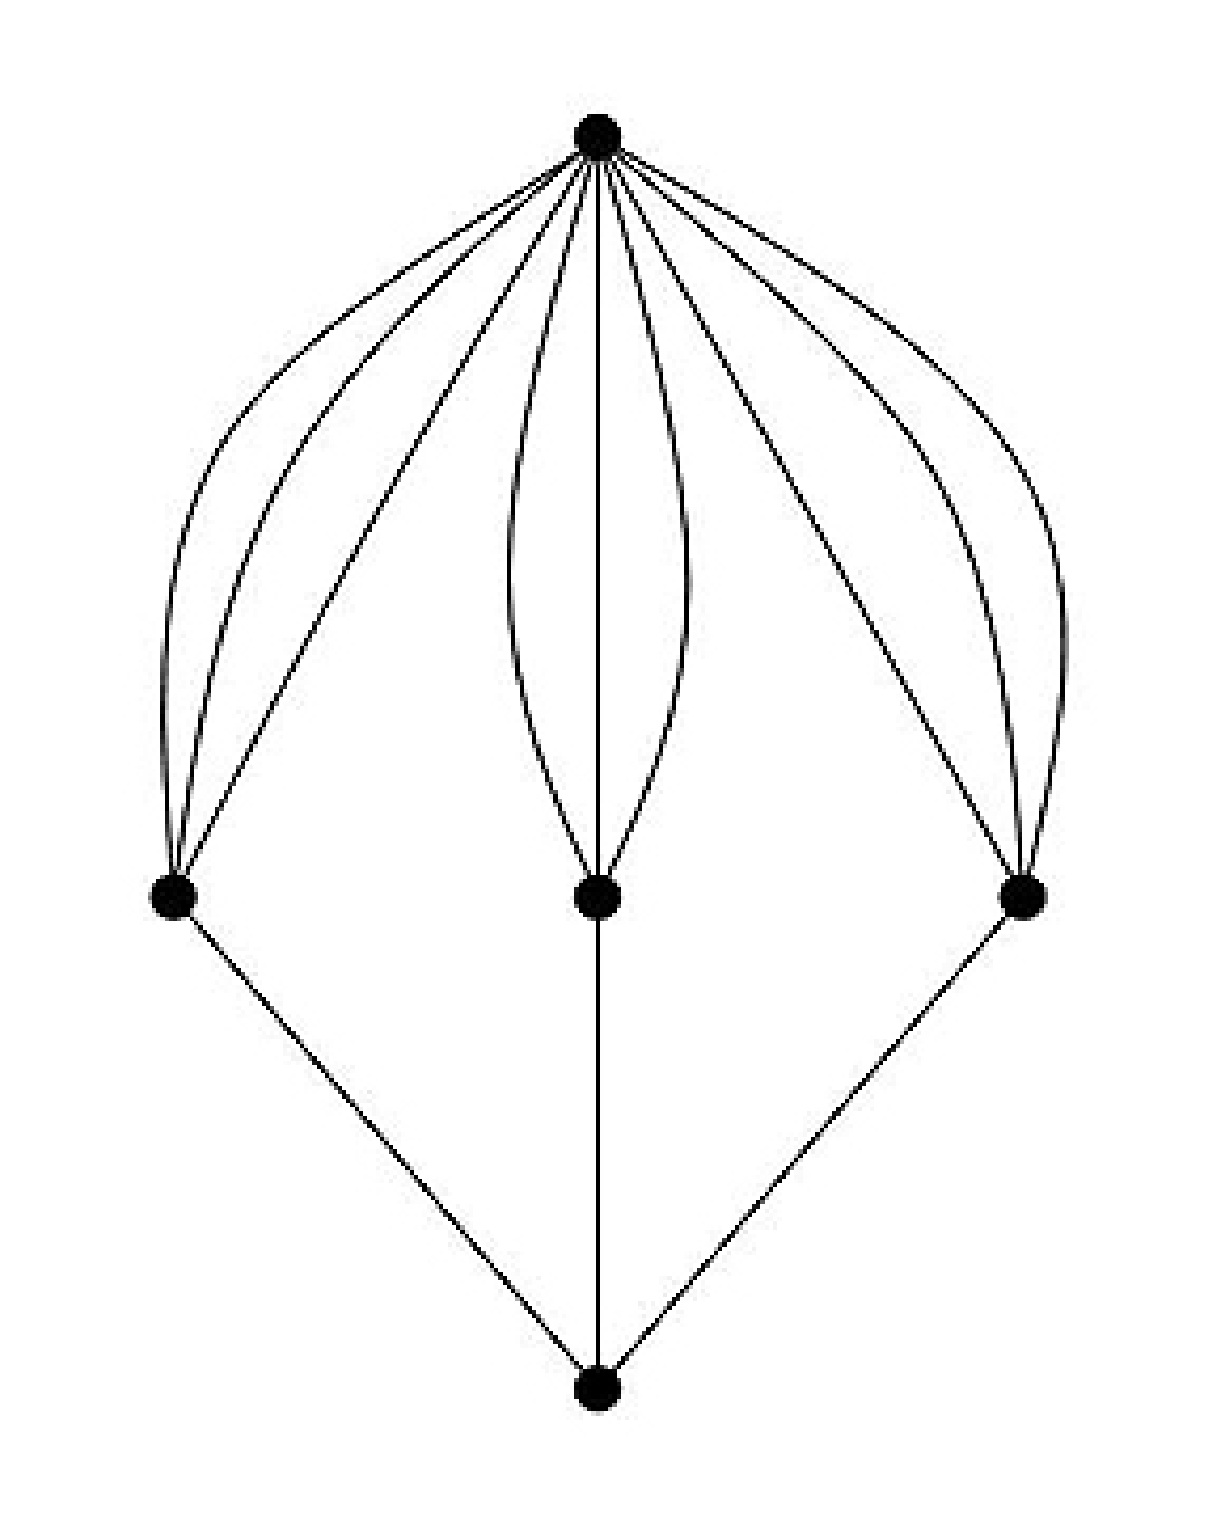
\includegraphics[width=15pc]{figures/parachute.eps}\\
\caption{Երկկողմանի մուլտիգրաֆ $Par(3,3,3)$:}\label{f3_parachute}
\end{center}
\end{figure}

$Par(r_{1},\ldots,r_{n})$-ը կապակցված երկկողմանի մուլտիգրաֆ է, որի համար $\vert V(Par(r_{1},\ldots,r_{n}))\vert=n+2$, $\Delta
(Par(r_{1},\ldots,r_{n}))=d(u)=\underset{i=1}{\overset{n}{\sum
}}r_{i}$, և $d(w)=n$, $d(v_{i})=r_{i}+1$, $i=1,2,\ldots,n$:

\begin{theorem}
\label{t3_parachute} Եթե $\underset{i=3}{\overset{n}{\sum }}r_{i}\geq
n+1$ ($n\geq 3$), ապա $Par(r_{1},\ldots,r_{n})\notin \mathfrak{N}$.
\end{theorem}
\begin{proof}[Ապացույց] Ենթադրենք հակառակը՝
$\alpha$-ն $Par(r_{1},\ldots,r_{n})$ մուլտիգրաֆի միջակայքային $t$-ներկում է ինչ որ $t$-ի համար. $t \geq \underset{i=1}{\overset{n}{\sum }}r_{i}$:

Դիտարկենք $u$ գագաթը: Ենթադրենք $v_{i_{0}}$-ը և $v_{i_{1}}$-ը $u$-ին հարևան այն գագաթներն են, որոնց համար 
$\alpha(uv_{i_{0}})=\underline{S}(u,\alpha)=s$ և
$\alpha(uv_{i_{1}})=\overline{S}(u,\alpha)=s+\underset{i=1}{\overset{n}{\sum
}}r_{i}-1$: Քանի որ $n\geq 3$, ունենք, որ $i_{0}\neq i_{1}$, և ըստ $Par(r_{1},\ldots,r_{n})$ մուլտիգրաֆի սահմանման ստանում ենք
\begin{center}
$\alpha(v_{i_{0}}w)\leq s+d(v_{i_{0}})-1=s+r_{i_{0}}$, ուստի
\end{center}
\begin{center}
$\alpha(v_{i_{1}}w)\leq s+r_{i_{0}}+d(w)-1=s+r_{i_{0}}+n-1$.
\end{center}

Հետևաբար՝
\begin{center}
$s+\underset{i=1}{\overset{n}{\sum
}}r_{i}-1=\alpha(uv_{i_{1}})=\overline{S}(u,\alpha)\leq
s+r_{i_{0}}+n-1+d(v_{i_{1}})-1=s+r_{i_{0}}+r_{i_{1}}+n-1$:
\end{center}

Փաստորեն ստացվում է, որ
\begin{center}
$\underset{i=3}{\overset{n}{\sum }}r_{i}\leq
\underset{i=1}{\overset{n}{\sum }}r_{i} - (r_{i_{0}}+r_{i_{1}})\leq
n$,
\end{center}
ինչը հակասություն է:
\end{proof}

Նկատենք, որ $Par(3,3,3)$ մուլտիգրաֆը չի բավարարում վերը նշված թեորեմի պայմաններին, սակայն այն ևս չունի միջակայքային ներկում:

\begin{remark}
\label{r3_parachute_333}
$Par(3,3,3) \notin \mathfrak{N}$
\end{remark}
\begin{proof}[Ապացույց]
Ցույց տանք, որ չնայած Նկ. \ref{f3_parachute}-ում պատկերված $Par(3,3,3)$ մուլտիգրաֆը չի բավարարում Թեորեմ \ref{t3_parachute}-ի պայմաններին, այն ևս միջակայքային ներկում չունի: Ենթադրենք հակառակը, դիցուք $\alpha$-ն $Par(3,3,3)$-ի որևէ միջակայքային ներկում է: Պահպանենք նախորդ թեորեմում ներմուծված գագաթների նշանակումները:

Դիցուք $S(u,\alpha)=[a,a+8]$: Առանց ընդհանրությունը խախտելու կարող ենք համարել, որ $a \in S(v_1,\alpha)$, իսկ $a+8 \in S(v_3, \alpha)$: $v_1, w, v_3$ գագաթների սպեկտրների միջակայք լինելը հնարավոր է ապահովել միայն այն դեպքում, երբ $S(v_1,\alpha)=[a,a+3]$, $S(w,\alpha)=[a+3,a+5]$, իսկ $S(v_3,\alpha)=[a+5,a+8]$: Սակայն այդ դեպքում մի կողմից ստանում ենք, որ $\alpha(uv_2)=5$, իսկ մյուս կողմից՝ $5$ գույնը պետք է օգտագործվի նաև $uv_2$ կողերից մեկի վրա, ինչը հակասություն է:
\end{proof}

Հաջորդ թեորեմից հետևում է, որ $Par(3,3,3)$ մուլտիգրաֆից ավելի փոքր թվով գագաթներով միջակայքային ներկում չունեցող երկկողմանի մուլտիգրաֆ գոյություն չունի:

\begin{theorem}
\label{t3_bipartite_multi_4} Եթե $G$-ն կապակցված երկկողմանի մուլտիգրաֆ է, ընդ որում $\vert V(G)\vert\leq 4$, ապա $G\in \mathfrak{N}$: Մյուս կողմից՝ ցանկացած դրական $n \geq 5$ թվի համար գոյություն ունի $G$ կապակցված երկկողմանի մուլտիգրաֆ, որի համար $|V(G)|=n$ և $G\notin \mathfrak{N}$:
\end{theorem}
\begin{proof}[Ապացույց]
Այն դեպքերը, երբ $\vert V(G)\vert\leq 3$ ակնհայտ են: Ենթադրենք $\vert
V(G)\vert= 4$. Եթե $G$-ի հիմքում ընկած գրաֆը ծառ է, ապացույցը նորից ակնհայտ է: Ուստի, ենթադրենք $V(G)=\{u,v,w,z\}$ և
$E(G)=E(uv)\cup E(vw)\cup E(wz)\cup E(uz)$, որտեղ $\mu(uv)=a$,
$\mu(vw)=b$, $\mu(wz)=c$, $\mu(uz)=d$: Առանց ընդհանրությունը խախտելու կարող ենք ենթադրել, որ ${\max} \{a,b,c,d\}=d$. Ներկենք $E(uv)$ կողերը
$d+1,\ldots,d+a$ գույներով, $E(vw)$ կողերը՝ 
$d-b+1,\ldots,d$, $E(wz)$ կողերը՝ $d+1,\ldots,d+c$,
իսկ $E(uz)$ կողերը՝ $1,\ldots,d$ գույներով: Եթե $a<c$, ապա ստացվածը $G$ մուլտիգրաֆի միջակայքային $(d+c)$-ներկում է: Հակառակ դեպքում, ստացվածը $G$ մուլտիգրաֆի միջակայքային $(d+a)$-ներկում է:

Թեորեմի երկրորդ մասը ցույց տալու համար նկատենք, որ ըստ Թեորեմ \ref{t3_parachute}-ի` ցանկացած $n \geq 3$ թվի համար $G_n = Par(\underbrace{n+1,\ldots,n+1}_{n})$ երկկողմանի մուլտիգրաֆը միջակայքային ներկում չունի, ընդ որում՝ $|V(G_n)|=n+2$:
\end{proof}

Պարագրաֆի վերջում ցույց տանք, որ բոլոր ենթախորանարդ երկկողմանի մուլտիգրաֆները միջակայքային ներկվող են:

\begin{theorem}
\label{t3_bipartite_multi_Delta3} Եթե $G$-ն երկկողմանի մուլտիգրաֆ է, որի համար
$\Delta(G)\leq 3$, ապա $G\in \mathfrak{N}$ և $w(G)\leq 4$: Մյուս կողմից՝ ցանկացած դրական $\Delta \geq 9$ թվի համար գոյություն ունի $G$ կապակցված երկկողմանի մուլտիգրաֆ, որի համար $\Delta(G)=\Delta$ և $G\notin \mathfrak{N}$:
\end{theorem}
\begin{proof}[Ապացույց] Ցույց տանք, որ եթե $G$-ն երկկողմանի մուլտիգրաֆ է, ընդ որում $\Delta(G)\leq 3$, ապա
$G$-ն ունի միջակայքային ներկում ոչ ավել քան չորս գույներով:

Ապացույցը կատարենք ինդուկցիայով ըստ $\vert E(G)\vert$-ի: Պնդումն ակնհայտ է, երբ $\vert E(G)\vert\leq 4$:
Ենթադրենք, որ $\vert E(G)\vert\geq 5$ և պնդումը ճիշտ է բոլոր այնպիսի $G^{\prime}$ երկկողմանի մուլտիգրաֆների համար, 
որոնց համար $\Delta(G^{\prime})\leq 3$ և $\vert
E(G^{\prime})\vert<\vert E(G)\vert$:

Դիտարկենք $G$ մուլտիգրաֆը: Այն կապակցված է: Եթե
$\Delta(G)\leq 2$, ապա $G\in \mathfrak{N}$ և $w(G)\leq 2$. Ենթադրենք, որ $\Delta(G)=3$. Եթե $G$-ն չունի պատիկ կողեր, ապա պնդումը հետևում է Թեորեմ \ref{t3_Hansen_Delta3}-ից: Ուստի ենթադրենք, որ $G$-ն ունի պատիկ կողեր:

Դիցուք $uv\in E(G)$ և $\mu(uv)\geq 2$. Եթե $\mu(uv)= 3$, ապա $G$-ն բաղկացած է միայն $u$ և $v$ գագաթներից և $uv$ երեք պատիկ կողերից, ուստի այն ունի միջակայքային $3$-ներկում: Այժմ ենթադրենք, որ $\mu(uv)= 2$: Դիտարկենք երկու դեպք.

Դեպք 1. $d_{G}(v)=2$ և $d_{G}(u)=\Delta(G)=3$:

Այս դեպքում գոյություն ունի $uw$ կող, որը հանդիսանում է կամուրջ
$G$-ում: Դիտարկենք $G^{\prime}=G-E(uv)$ մուլտիգրաֆը, որտեղ
$E(uv)=\{e_{1},e_{2}\}$. Ինդուկցիոն ենթադրության համաձայն, $G^{\prime}$-ը ունի $\alpha$ միջակայքային ներկում ոչ ավել քան չորս գույներով:
Առանց ընդհանրությունը խախտելու կարող ենք համարել, որ $\alpha (uw)\leq 2$ (հակառակ դեպքում կդիտարկենք $\beta(e)=4-\alpha(e)$ կամ
$\beta(e)=5-\alpha(e)$ ներկումը ցանկացած $e\in E(G^{\prime})$ կողի համար): Այժմ ներկենք $e_{i}$ կողը $\alpha (uw)+i$, գույնով, $i=1,2$: Դժվար չէ համոզվել, որ ստացված ներկումը $G$ մուլտիգրաֆի միջակայքային ներկում է ոչ ավել քան չորս գույներով:

Դեպք 2. $d_{G}(u)=d_{G}(v)=\Delta(G)=3$:

Այս դեպքում $G$-ում գոյություն ունեն $x,y$ գագաթներ ($x\neq y$), այնպես, որ $ux\in E(G)$ և $vy\in E(G)$: Դիտարկենք $G^{\prime}=(G-E(uv)-ux-vy)+xy$ մուլտիգրաֆը, որտեղ $E(uv)=\{e_{1},e_{2}\}$: Ինդուկցիոն ենթադրության համաձայն, $G^{\prime}$-ը ունի $\alpha$ միջակայքային ներկում ոչ ավել քան չորս գույներով:
Առանց ընդհանրությունը խախտելու կարող ենք համարել, որ $\alpha (xy)\leq 2$ (հակառակ դեպքում կդիտարկենք $\beta(e)=4-\alpha(e)$ կամ
$\beta(e)=5-\alpha(e)$ ներկումը ցանկացած $e\in E(G^{\prime})$ կողի համար): Այնուհետև ջնջենք $xy$ կողը և ներկենք $ux$ և $vy$ կողերը
$\alpha (xy)$ գույնով, իսկ $e_{i}$ կողը՝ $\alpha (xy)+i$ գույնով,
$i=1,2$: Հեշտ է տեսնել, որ ստացված ներկումը $G$ մուլտիգրաֆի միջակայքային ներկում է ոչ ավել քան չորս գույներով:

Թեորեմի երկրորդ մասի ապացույցը անմիջապես հետևում է Պնդում \ref{r3_parachute_333}-ից և Թեորեմ \ref{t3_parachute}-ից:
\end{proof}